% !TeX program = xelatex
\documentclass[a4paper,10pt]{article}

% ============================================================================
% កញ្ចប់បណ្ណាល័យ (Packages) – តាមលំនាំស្តង់ដារ អនុវិទ្យាល័យព្រះក្រសាំង (ls_plan.tex)
% បរិបទ៖ ថ្នាក់រៀនគ្មានស្លាយ LCD – បង្រៀនដោយប្រើក្ដារខៀន សៀវភៅគោល និងសន្លឹកកិច្ចការស-ខ្មៅ
% ============================================================================
\usepackage[a4paper, left=0.95cm, right=0.95cm, top=0.85cm, bottom=0.92cm, footskip=0.52cm]{geometry}
\usepackage{amsmath}
\usepackage{unicode-math}
\usepackage{fontspec}
\usepackage{array, longtable, multirow, colortbl}
\usepackage[table]{xcolor}
\usepackage{enumitem}
\usepackage{pifont}
\usepackage{fancyhdr}
\usepackage{tikz}
\usetikzlibrary{calc, arrows.meta, positioning, patterns, babel}

\makeatletter
\let\@expl@@@mark@update@singlecol@structures@@\relax
\makeatother

\providecommand{\NGSFindFonts}{%
  \IfFileExists{C:/Windows/Fonts/cambria.ttc}{%
    \def\NGSSysPath{C:/Windows/Fonts/}%
    \def\NGSUserPath{C:/Users/KIT/AppData/Local/Microsoft/Windows/Fonts/}%
  }{%
    \IfFileExists{./fonts/KhmerOSsiemreap.ttf}{\def\NGSSysPath{./fonts/}\def\NGSUserPath{./fonts/}}{%
    \IfFileExists{../fonts/KhmerOSsiemreap.ttf}{\def\NGSSysPath{../fonts/}\def\NGSUserPath{../fonts/}}{%
    \IfFileExists{../../fonts/KhmerOSsiemreap.ttf}{\def\NGSSysPath{../../fonts/}\def\NGSUserPath{../../fonts/}}{%
    \IfFileExists{../../../fonts/KhmerOSsiemreap.ttf}{\def\NGSSysPath{../../../fonts/}\def\NGSUserPath{../../../fonts/}}{%
    \IfFileExists{../../../../fonts/KhmerOSsiemreap.ttf}{\def\NGSSysPath{../../../../fonts/}\def\NGSUserPath{../../../../fonts/}}{%
    \IfFileExists{../../../../../fonts/KhmerOSsiemreap.ttf}{\def\NGSSysPath{../../../../../fonts/}\def\NGSUserPath{../../../../../fonts/}}{%
    \IfFileExists{../../../../../../fonts/KhmerOSsiemreap.ttf}{\def\NGSSysPath{../../../../../../fonts/}\def\NGSUserPath{../../../../../../fonts/}}{%
      \def\NGSSysPath{../../../../../../../fonts/}\def\NGSUserPath{../../../../../../../fonts/}%
    }}}}}}}%
  }%
}
\NGSFindFonts

\setmathfont[Path={\NGSSysPath}, FontIndex=1, Scale=1.02]{cambria.ttc}
\defaultfontfeatures{Ligatures=TeX}

\setmainfont[
  Path={\NGSUserPath},
  Extension=.ttf,
  Script=Khmer,
  BoldFont={KhmerOSsiemreap},
  BoldFeatures={FakeBold=1.8},
  ItalicFont={KhmerOSsiemreap},
  ItalicFeatures={FakeSlant=0.25},
  BoldItalicFont={KhmerOSsiemreap},
  BoldItalicFeatures={FakeBold=1.8, FakeSlant=0.25}
]{KhmerOSsiemreap}

\newfontfamily\muol[Path={\NGSUserPath}, Extension=.ttf, Script=Khmer]{KhmerOSmuollight}
\newfontfamily\TimesEn[Path={\NGSSysPath}, Extension=.ttf, BoldFont={timesbd}, ItalicFont={timesi}, BoldItalicFont={timesbi}]{times}
\newfontfamily\NagaBold[Path={\NGSUserPath}, Extension=.ttf]{AKbalthom Naga Bold}
\newfontfamily\CalibriFont[Path={\NGSSysPath}, Extension=.ttf]{calibri}
\newfontfamily\Tacteing[Path={\NGSUserPath}]{TACTENG.TTF}
\newfontfamily\CourierBullet[Path={\NGSSysPath}, Extension=.ttf]{cour}
\newcommand{\wcirc}{{\CourierBullet\fontsize{9.5pt}{11pt}\selectfont o}}

\XeTeXlinebreaklocale "km"
\XeTeXlinebreakskip = 0pt plus 1pt minus 0.1pt

\definecolor{stepgray}{HTML}{D9D9D9}
\definecolor{headgray}{HTML}{F2F2F2}
\definecolor{boxgray}{HTML}{D9D9D9}
\definecolor{darkred}{HTML}{C00000}
\definecolor{red5e}{HTML}{FF0000}

\pagestyle{fancy}
\fancyhf{}
\renewcommand{\headrulewidth}{0pt}
\fancyfoot[R]{\CalibriFont\fontsize{11pt}{13pt}\selectfont\thepage}

\setlength{\parindent}{0pt}
\setlength{\parskip}{0pt}
\setlength{\tabcolsep}{3.8pt}

\newcolumntype{L}[1]{>{\raggedright\arraybackslash}p{#1}}

\newcommand{\en}[1]{{\TimesEn #1}}
\newcommand{\enbf}[1]{{\TimesEn\textbf{#1}}}
\newcommand{\unit}[1]{\,\text{\en{#1}}}
\newcommand{\fiveE}[1]{{\NagaBold\fontsize{9.5pt}{13pt}\selectfont\textcolor{red5e}{#1}}}
\newcommand{\timenote}[1]{\textcolor{darkred}{\textit{#1}}}
\newcommand{\graybox}[1]{\colorbox{boxgray}{\strut\hspace{2pt}#1\hspace{2pt}}}
\newcommand{\ditem}{\tikz[baseline=-0.5ex]\fill (0,0.42ex) -- (0.42ex,0) -- (0,-0.42ex) -- (-0.42ex,0) -- cycle;\hspace{0.3em}}
\newcommand{\cnum}[1]{{\fontsize{10.5pt}{12pt}\selectfont\ding{\numexpr171+#1\relax}}\hspace{0.2em}}
\newcommand{\cfig}[1]{\par\vspace{4pt}{\centering #1\par}\vspace{4pt}}
\newcommand{\stepheader}[1]{\multicolumn{3}{|c|}{\cellcolor{stepgray}\muol #1} \\* \noalign{\hrule height 0.4pt}}
\newcommand{\khmflourish}{{\Tacteing\fontsize{36pt}{14pt}\selectfont\raisebox{-5pt}{3}}}

% ============================================================================
% ម៉ាក្រូរូបភាពគរុកោសល្យស-ខ្មៅ (Proportional B&W TikZ Diagrams)
% ============================================================================

% ១. E1/E2: ប្រៀបធៀបបន្ទះចតុកោណកែងបូកចូលគ្នា (b+2b+3b=6b, ទំ.៥៣) vs សួនច្បារគុណគ្នា (5x * 2x = 10x^2, ទំ.៥៤)
\newcommand{\figContrastALGTwo}{%
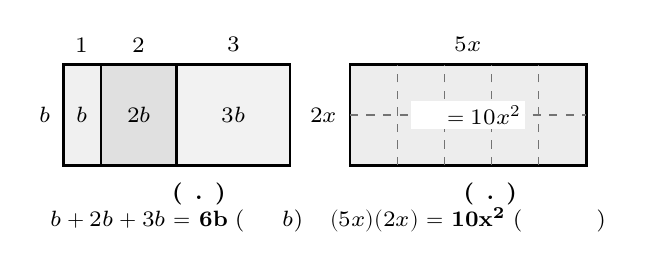
\begin{tikzpicture}[scale=0.80, every node/.style={font=\footnotesize, text=black}]
  % ឆ្វេង៖ ការបូកផ្ទៃក្រឡាបន្ទះចតុកោណកែង b + 2b + 3b = 6b (ទំ.៥៣)
  \begin{scope}[shift={(0,0)}]
    \draw[black, line width=0.95pt, fill=gray!12] (0,0.35) rectangle (0.60,1.95);
    \draw[black, line width=0.95pt, fill=gray!24] (0.60,0.35) rectangle (1.80,1.95);
    \draw[black, line width=0.95pt, fill=gray!10] (1.80,0.35) rectangle (3.60,1.95);
    \node[left=1pt] at (0,1.15) {$b$};
    \node[above=1pt] at (0.30,1.95) {$1$};
    \node[above=1pt] at (1.20,1.95) {$2$};
    \node[above=1pt] at (2.70,1.95) {$3$};
    \node at (0.30,1.15) {$b$};
    \node at (1.20,1.15) {$2b$};
    \node at (2.70,1.15) {$3b$};
    \node[anchor=north, text width=3.55cm, align=center] at (1.80,0.22) {\textbf{វិធីបូក (ទំ.៥៣)៖}\\$b+2b+3b = \mathbf{6b}$ (រក្សា $b$)};
  \end{scope}

  % ស្ដាំ៖ ផ្ទៃក្រឡាសួនច្បារ (5x)(2x) = 10x^2 (ទំ.៥៤)
  \begin{scope}[shift={(4.55,0)}]
    \draw[black, line width=1.0pt, fill=gray!14] (0,0.35) rectangle (3.75,1.95);
    \foreach \x in {0.75, 1.50, 2.25, 3.00} {
      \draw[black!55, line width=0.45pt, dashed] (\x,0.35) -- (\x,1.95);
    }
    \draw[black!55, line width=0.45pt, dashed] (0,1.15) -- (3.75,1.15);
    \node[left=1pt] at (0,1.15) {$2x$};
    \node[above=1pt] at (1.875,1.95) {$5x$};
    \node[fill=white, inner sep=1.5pt] at (1.875,1.15) {ផ្ទៃ $= 10x^2$};
    \node[anchor=north, text width=3.80cm, align=center] at (1.875,0.22) {\textbf{វិធីគុណ (ទំ.៥៤)៖}\\$(5x)(2x) = \mathbf{10x^2}$ (បូកនិទស្សន្ត)};
  \end{scope}
\end{tikzpicture}}

% ២. E4: ប្លង់ភូមិគ្រឹះ 18a x 12a (ទំ.៥៥) និងស្រះឈូកផ្ទៃ 16xy^2 ទទឹង 4y (ទំ.៥៥)
\newcommand{\figModelsALGTwo}{%
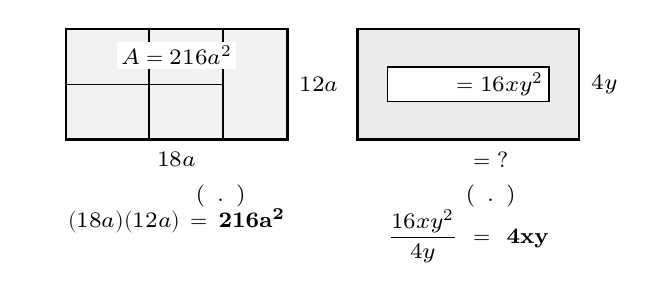
\begin{tikzpicture}[scale=0.78, every node/.style={font=\footnotesize, text=black}]
  % ឆ្វេង៖ ប្លង់ភូមិគ្រឹះ 18a x 12a (ទំ.៥៥)
  \begin{scope}[shift={(0,0)}]
    \draw[black, line width=1.0pt, fill=gray!10] (0,0.35) rectangle (3.60,2.15);
    \draw[black, line width=0.6pt] (1.35,0.35) -- (1.35,2.15);
    \draw[black, line width=0.6pt] (0,1.25) -- (2.55,1.25);
    \draw[black, line width=0.6pt] (2.55,0.35) -- (2.55,2.15);
    \node[below=1pt] at (1.80,0.35) {$18a$};
    \node[right=1pt] at (3.60,1.25) {$12a$};
    \node[fill=white, inner sep=1.5pt] at (1.80,1.72) {$A = 216a^2$};
    \node[anchor=north, text width=3.55cm, align=center] at (1.80,-0.22) {ប្លង់ភូមិគ្រឹះ (ទំ.៥៥)៖\\$(18a)(12a) = \mathbf{216a^2}$};
  \end{scope}

  % ស្ដាំ៖ ស្រះទឹករាងចតុកោណកែង ផ្ទៃ 16xy^2 ទទឹង 4y (ទំ.៥៥)
  \begin{scope}[shift={(4.75,0)}]
    \draw[black, line width=1.0pt, fill=gray!16] (0,0.35) rectangle (3.60,2.15);
    \node[fill=white, draw=black, line width=0.5pt, inner sep=2pt] at (1.80,1.25) {ផ្ទៃក្រឡា $= 16xy^2$};
    \node[right=1pt] at (3.60,1.25) {$4y$};
    \node[below=1pt] at (1.80,0.35) {បណ្ដោយ $= \text{?}$};
    \node[anchor=north, text width=3.80cm, align=center] at (1.80,-0.22) {ស្រះទឹក (ទំ.៥៥)៖\\$\dfrac{16xy^2}{4y} = \mathbf{4xy}$};
  \end{scope}
\end{tikzpicture}}

\begin{document}
\fontsize{10pt}{15.2pt}\selectfont

% -------------------- ក្បាលកិច្ចតែងការ (Header) --------------------
\begin{center}
  {\muol\fontsize{11pt}{16pt}\selectfont ព្រះរាជាណាចក្រកម្ពុជា}\\[2pt]
  {\muol\fontsize{10pt}{15pt}\selectfont ជាតិ សាសនា ព្រះមហាក្សត្រ}\\[1pt]
  \khmflourish
\end{center}

\vspace{-28pt}
{\muol\fontsize{9.5pt}{12.5pt}\selectfont
មន្ទីរអប់រំ យុវជន និងកីឡា ខេត្តកំពង់ធំ\\
ការិយាល័យអប់រំ យុវជន និងកីឡា ស្រុកកំពង់ស្វាយ\\
អនុវិទ្យាល័យព្រះក្រសាំង}

\vspace{1pt}
\begin{center}
  {\muol\fontsize{10pt}{14pt}\selectfont កិច្ចតែងការបង្រៀន}
\end{center}
\vspace{0pt}

% -------------------- ព័ត៌មានទូទៅ (Metadata) --------------------
{\renewcommand{\arraystretch}{0.95}
\hspace*{4.05cm}%
\begin{tabular}{@{}l l l@{}}
  - \hspace{0.35cm} មុខវិជ្ជា & : & គណិតវិទ្យា ថ្នាក់ទី៨ \\
  - \hspace{0.35cm} ចំណងជើងមេរៀន & : & មេរៀនទី៥ កន្សោមពីជគណិត \\
  - \hspace{0.35cm} ចំណងជើងរង & : & ១.៤--១.៦ ប្រមាណវិធីបូក ដក គុណ និងចែកឯកធា (ទំ.៥៣--៥៦) \\
  - \hspace{0.35cm} រយៈពេល & : & ១ ម៉ោងសិក្សា (៥០ នាទី) \\
  - \hspace{0.35cm} បង្រៀនដោយ & : & ហុក ប៊ុនថែន \\
  - \hspace{0.35cm} កាលបរិច្ឆេទ & : & ថ្ងៃសៅរ៍ ១១រោច ខែកត្តិក ព.ស.២៥៧០ (៥ ធ្នូ ២០២៦) \\
\end{tabular}
}

\vspace{1pt}

% -------------------- I. វត្ថុបំណង --------------------
\textbf{I.} {\muol វត្ថុបំណង}\\[1pt]
\hspace*{0.55cm}%
\begin{tabular}{@{}l l L{14.2cm}@{}}
  \wcirc \hspace{0.25cm} វិជ្ជាសម្បទា & : & សិស្សប្រាប់បានត្រឹមត្រូវនូវវិធានគណនាផលបូក និងផលដក \textbf{ឯកធាដូចគ្នា} (បូក/ដកតែមេគុណ រក្សាផ្នែកអថេរដដែល) ព្រមទាំងវិធានគុណ និងចែកឯកធា (គុណ/ចែកមេគុណនឹងមេគុណ ហើយបូក/ដកនិទស្សន្តតាមអថេរដូចគ្នា) តាមសៀវភៅគោល ទំ.៥៣--៥៦ ។ \\
  \wcirc \hspace{0.25cm} បំណិនសម្បទា & : & សិស្សគណនាផលបូក ផលដក ផលគុណ និងផលចែកឯកធា ព្រមទាំងដោះស្រាយលំហាត់ផ្ទៃក្រឡាសួនច្បារ ប្លង់ភូមិគ្រឹះ និងស្រះទឹកលើសន្លឹកកិច្ចការស-ខ្មៅដោយមិនច្រឡំបូកនិទស្សន្តពេលធ្វើវិធីបូកឡើយ ។ \\
  \wcirc \hspace{0.25cm} ចរិយាសម្បទា & : & សិស្សមានស្មារតីប្រុងប្រយ័ត្នខ្ពស់ក្នុងការផ្ទៀងផ្ទាត់សញ្ញា និងនិទស្សន្តមុនធ្វើប្រមាណវិធី និងចូលរួមផ្ទៀងផ្ទាត់ចម្លើយគ្នាប្រកបដោយភាពស្មោះត្រង់ ។ \\
\end{tabular}

\vspace{1pt}

% -------------------- II. សម្ភារៈឧបទេស --------------------
\textbf{II.} {\muol សម្ភារៈឧបទេស}\\[1pt]
\hspace*{0.55cm}$\bullet$ \hspace{0.35cm} សៀវភៅសិក្សាគោលគណិតវិទ្យាថ្នាក់ទី៨ (ទំ.៥៣--៥៦ និងទំ.៧២--៧៣) ក្ដារខៀន ដីស បន្ទាត់ និងសន្លឹកកិច្ចការសិស្សស-ខ្មៅ (\en{Worksheet\_ALG52} ចំនួន ២ ទំព័រ \en{A4} ដោយគ្មានស្លាយ \en{LCD}) ។

\vspace{1pt}

% -------------------- III. វិធីសាស្រ្តបង្រៀន --------------------
\textbf{III.} {\muol វិធីសាស្រ្តបង្រៀន}\\[1pt]
\hspace*{0.55cm}$\bullet$ \hspace{0.35cm} គោលវិធីសិស្សមជ្ឈមណ្ឌលតាមគំរូ \en{5Es} រួមបញ្ចូល \textbf{តារាងប្រៀបធៀបផ្ទុយគ្នារវាងគំរូបន្ទះផ្ទៃក្រឡា និងគំរូចតុកោណកែង} (\en{Contrasting Area-Strip vs.\ Rectangle-Area Matrix}; \en{Aydin-G\"u\c{c} \& Ayg\"un, 2021; Moru \& Mathunya, 2022}) ដើម្បីបំបាត់ការយល់ច្រឡំ $2xy+5xy=7x^2y^2$ ។

\vspace{2pt}

% -------------------- IV. ដំណើរការបង្រៀន --------------------
\textbf{IV.} {\muol ដំណើរការបង្រៀន}\\[-6pt]

{\renewcommand{\arraystretch}{1.15}
\begin{longtable}{|L{5.50cm}|L{7.90cm}|L{4.80cm}|}
\hline
\multicolumn{1}{|c|}{\cellcolor{headgray}\muol សកម្មភាពគ្រូ} &
\multicolumn{1}{c|}{\cellcolor{headgray}\muol ខ្លឹមសារមេរៀន} &
\multicolumn{1}{c|}{\cellcolor{headgray}\muol សកម្មភាពសិស្ស} \\[2pt]
\hline
\endfirsthead

\hline
\multicolumn{1}{|c|}{\cellcolor{headgray}\muol សកម្មភាពគ្រូ} &
\multicolumn{1}{c|}{\cellcolor{headgray}\muol ខ្លឹមសារមេរៀន} &
\multicolumn{1}{c|}{\cellcolor{headgray}\muol សកម្មភាពសិស្ស} \\[2pt]
\hline
\endhead

\hline
\endfoot

% ==================== ជំហានទី១ (2min) ====================
\stepheader{ជំហានទី១ ៖ រដ្ឋបាលថ្នាក់ (២ នាទី)}
$\bullet$ ពិនិត្យអវត្តមាន សណ្ដាប់ធ្នាប់ អនាម័យ និងសៀវភៅគោល \par\vspace{1pt}
$\bullet$ ចែកសន្លឹកកិច្ចការស-ខ្មៅ \en{Worksheet\_ALG52} ដល់សិស្សគ្រប់គ្នា
&
$\bullet$ វត្តមានសិស្ស ឯកសណ្ឋាន និងសណ្ដាប់ធ្នាប់ថ្នាក់រៀន \par
$\bullet$ សន្លឹកកិច្ចការសិស្ស \en{Worksheet\_ALG52} (ទំព័រ ១--២) លើតុរៀងៗខ្លួន
&
$\circ$ ប្រធានថ្នាក់រាយការណ៍អវត្តមាន \par
$\circ$ បំពេញឈ្មោះលើសន្លឹកកិច្ចការ \\
\hline

% ==================== ជំហានទី២ (9min) ====================
\stepheader{ជំហានទី២ ៖ កែកិច្ចការផ្ទះ រំលឹកមេរៀនចាស់ និងភ្ជាប់បញ្ហាថ្មី (៩ នាទី)}
\ditem \textbf{កែកិច្ចការផ្ទះ ($\le 3\unit{min}$)៖} \par
$\bullet$ ហៅសិស្ស ១ រូបឡើងកែលំហាត់ទី១ (ទំ.៧២) លើក្ដារខៀន
&
\textbf{កំណែកិច្ចការផ្ទះ (លំហាត់ទី១ ទំ.៧២)៖} \par
$\bullet$ \textbf{ជាឯកធា៖} $\frac{x^3}{3}$ (មេគុណ $\frac{1}{3}$, ដឺក្រេ $3$); $\sqrt{5}ax^2$ (មេគុណ $\sqrt{5}$, ដឺក្រេ $3$); $\frac{7xy^2}{3}$ (មេគុណ $\frac{7}{3}$, ដឺក្រេ $3$) ។ \par
$\bullet$ \textbf{មិនមែនឯកធា៖} $x+2y$, $\frac{a}{x^2}$, និង $x(x+y)=x^2+xy$ ។
&
$\circ$ ផ្ទៀងផ្ទាត់មេគុណប្រភាគ $\frac{1}{3}, \frac{7}{3}$ និងកែសម្រួលចម្លើយ \\[3pt]

\ditem \textbf{រំលឹកមេរៀនចាស់ ($3\unit{min}$)៖} \par
$\bullet$ សួររំលឹករូបមន្តគុណ និងចែកស្វ័យគុណមានគោលដូចគ្នា ($a^m\cdot a^n$ និង $\frac{a^m}{a^n}$) ព្រមទាំងលក្ខណៈចែកចាយ $(m+n)k$
&
\textbf{សំណួររំលឹកច្បាប់ស្វ័យគុណ (មេរៀនទី២)៖} \par
១) $a^m \cdot a^n = a^{m+n}$ \quad និង \quad $\dfrac{a^m}{a^n} = a^{m-n}$ ($a\ne 0$) ។ \par
២) លក្ខណៈចែកចាយ៖ $mb + nb = (m+n)b$ ។
&
$\circ$ ឆ្លើយរំលឹករូបមន្តបូក និងដកនិទស្សន្តពេលគុណ និងចែកស្វ័យគុណ \\[3pt]

\fiveE{E1 - Engage} \timenote{(3 នាទី)} \par\vspace{1pt}
$\bullet$ សរសេរគូប្រមាណវិធីភ្លោះ $2xy + 5xy$ និង $(2x)(5y)$ លើក្ដារខៀន រួចឱ្យសិស្សគូសធីកការទស្សន៍ទាយក្នុងផ្នែកទី១
&
\textbf{ស្ថានភាពភ្ជាប់បញ្ហា៖ អន្ទាក់និទស្សន្តពេលបូក ទល់នឹងពេលគុណ!} \par
សិស្សពីរនាក់ប្រកែកគ្នា៖ សុខថា $2xy + 5xy = 7x^2y^2$ ចំណែកធីតាថា $2xy + 5xy = 7xy$ ។ ចុះបើគណនាផ្ទៃសួនច្បារ $(5x)(2x)$ វិញ តើស្មើ $10x$ ឬ $10x^2$? \par
\hspace*{0.3em}– \textbf{សំណួរបេសកកម្ម៖} «ហេតុអ្វីពេលបូកឯកធាដូចគ្នា និទស្សន្ត \textbf{មិនផ្លាស់ប្ដូរ} តែពេលគុណឯកធា និទស្សន្តបែរជា \textbf{បូកបញ្ចូលគ្នា}?»
&
$\circ$ គិតពិចារណាលើកំហុស $7x^2y^2$ \par
$\circ$ គូសធីកការទស្សន៍ទាយមុនរៀនក្នុងប្រអប់ផ្នែកទី១ នៃសន្លឹកកិច្ចការ \\[3pt]

& \cfig{\figContrastALGTwo} & \\
\hline

% ==================== ជំហានទី៣ (17min) ====================
\stepheader{ជំហានទី៣ ៖ មេរៀនថ្មី — ប្រមាណវិធីបូក ដក គុណ និងចែកឯកធា (១៧ នាទី)}
\fiveE{E2 - Explore} \timenote{(11 នាទី)} \par\vspace{1pt}
\ditem \textbf{សកម្មភាពទី១៖ រុករកវិធីបូក-ដកឯកធាដូចគ្នាតាមផ្ទៃបន្ទះ ($5\unit{min}$)៖} \par
$\bullet$ ឱ្យសិស្សធ្វើការជាដៃគូលើ \textbf{ផ្នែកទី២ (ក)} នៃ \en{Worksheet\_ALG52} តាមរូបបន្ទះចតុកោណកែង ទំ.៥៣
&
\textbf{ការរុករកទី១ (១.៤ បូក និងដកឯកធាដូចគ្នា ទំ.៥៣)៖} \par
$\bullet$ បន្ទះចតុកោណកែង ៣ មានកម្ពស់ $b$ ដូចគ្នា និងទទឹង $1, 2, 3$ ដាក់តម្រៀបជាប់គ្នា បានទទឹងសរុប $1+2+3=6$ និងកម្ពស់នៅតែ $b$ ដដែល៖
\[ b + 2b + 3b = (1 + 2 + 3)b = \mathbf{6b} \quad (\text{មិនមែន } 6b^3 \text{ ទេ!}) \]
$\bullet$ ដូចគ្នាដែរ ចំពោះផលដក៖ $5x - 2x = (5 - 2)x = \mathbf{3x}$ ។
&
$\circ$ សង្កេតរូបបន្ទះចតុកោណកែង រួចទាញបានថាផ្នែកអថេរ $b$ រក្សាទុកដដែលពេលបូក/ដក \\[3pt]

\ditem \textbf{សកម្មភាពទី២៖ រុករកវិធីគុណ និងចែកឯកធា ($6\unit{min}$)៖} \par
$\bullet$ ឱ្យដៃគូបន្តបំពេញ \textbf{ផ្នែកទី២ (ខ)}៖ គណនាផ្ទៃសួនច្បារ (ទំ.៥៤) និងបណ្ដោយស្រះទឹក (ទំ.៥៥) ដោយពន្លាតជាកត្តា រួចទាញរូបមន្តខ្លី
&
\textbf{ការរុករកទី២ (១.៥ វិធីគុណ និង ១.៦ វិធីចែកឯកធា ទំ.៥៤--៥៥)៖} \par
$\bullet$ \textbf{វិធីគុណ៖} $(5x)(2x) = (5\cdot 2)(x\cdot x) = \mathbf{10x^2}$ ហើយ $(4x^2yc^4)(3xy^3c) = (4\cdot 3)(x^{2+1})(y^{1+3})(c^{4+1}) = \mathbf{12x^3y^4c^5}$ ។ \par
$\bullet$ \textbf{វិធីចែក៖} បណ្ដោយស្រះទឹក $= \dfrac{16xy^2}{4y} = \dfrac{16}{4} \cdot x \cdot y^{2-1} = \mathbf{4xy}$ និង $(8x^4y^5)\div(16x^2y^3) = \dfrac{8}{16}x^{4-2}y^{5-3} = \mathbf{\dfrac{1}{2}x^2y^2}$ ។
&
$\circ$ ផ្ដុំមេគុណនឹងមេគុណ និងអថេរដូចគ្នានឹងអថេរដូចគ្នា \par
$\circ$ សម្គាល់ការសម្រួលប្រភាគ $\frac{8}{16}=\frac{1}{2}$ \\[3pt]

\fiveE{E3 - Explain} \timenote{(6 នាទី)} \par\vspace{1pt}
$\bullet$ ហៅតំណាងដៃគូឡើងបកស្រាយ រួចគ្រូសង្ខេបតារាងប្រៀបធៀបវិធានទាំង ៣ និងធនាគារហេតុផល \cnum{1}--\cnum{4} លើក្ដារខៀន
&
\textbf{សង្ខេបវិធានប្រមាណវិធីលើឯកធា (សៀវភៅគោល ទំ.៥៤--៥៥)៖} \par
$\bullet$ \textbf{១.៤ បូក/ដកឯកធាដូចគ្នា (\cnum{1})៖} ធ្វើប្រមាណវិធីបូក ឬដក \textbf{តែផ្នែកមេគុណ} រួចគុណលទ្ធផលនឹងផ្នែកអថេរដដែល ($ma^k \pm na^k = (m\pm n)a^k$) ។ \textit{(ឯកធាមិនដូចគ្នា មិនអាចបូកបង្រួមចូលគ្នាបានទេ!)} \par
$\bullet$ \textbf{១.៥ វិធីគុណឯកធា (\cnum{2})៖} ផ្ដុំគុណមេគុណនឹងមេគុណ ហើយគុណផ្នែកអថេរនឹងផ្នែកអថេរដោយ \textbf{បូកនិទស្សន្ត} ($a^m\cdot a^n = a^{m+n}$) ។ \par
$\bullet$ \textbf{១.៦ វិធីចែកឯកធា (\cnum{3})៖} ចែកមេគុណនឹងមេគុណ ហើយចែកផ្នែកអថេរដោយ \textbf{ដកនិទស្សន្ត} ($\frac{a^m}{a^n} = a^{m-n}$) ។ (\cnum{4} បើនិទស្សន្តស្មើគ្នា សម្រួលអស់ស្មើ $1$៖ $\frac{y}{y}=1$) ។
&
$\circ$ ឡើងបង្ហាញការប្រៀបធៀបវិធានបូក និងគុណ \par
$\circ$ កត់ត្រាវិធាន \cnum{1}--\cnum{4} ចូលក្នុងប្រអប់ផ្នែកទី៣ នៃសន្លឹកកិច្ចការ \\
\hline

% ==================== ជំហានទី៤ (20min) ====================
\stepheader{ជំហានទី៤ ៖ ពង្រីកចំណេះដឹង និងវាយតម្លៃលទ្ធផលសិក្សា (២០ នាទី)}
\fiveE{E4 - Elaborate} \timenote{(10 នាទី)} \par\vspace{1pt}
\ditem \textbf{លំហាត់គំរូបូក-ដក និងប្លង់ភូមិគ្រឹះ (ទំ.៥៤--៥៥, $5\unit{min}$)៖} \par
$\bullet$ ដឹកនាំសិស្សដោះស្រាយលំហាត់គំរូទំ.៥៤--៥៥ ក្នុង \textbf{ផ្នែកទី៤ (១--២)} ដោយរំលឹកមេគុណលាក់មុខ $1$ និងសញ្ញាដក
&
\textbf{លំហាត់គំរូទី១ (បូក-ដក ទំ.៥៤) និងទី២ (ប្លង់ភូមិគ្រឹះ ទំ.៥៥)៖} \par
$\bullet$ \textbf{បូក-ដក៖} ខ) $3ab^2 + 7ab^2 + ab^2 = (3+7+\mathbf{1})ab^2 = \mathbf{11ab^2}$ \par
\hspace*{0.3em}គ) $8x^2y^3z - 3x^2y^3z - 7x^2y^3z = (8-3-7)x^2y^3z = \mathbf{-2x^2y^3z}$ \par
\hspace*{0.3em}ឃ) $10x^2y + x^2y - 5x^2y = (10+\mathbf{1}-5)x^2y = \mathbf{6x^2y}$ ។ \par
$\bullet$ \textbf{ផ្ទៃប្លង់ភូមិគ្រឹះ៖} $A = (18a)(12a) = (18\cdot 12)(a\cdot a) = \mathbf{216a^2}$ ឯកតាផ្ទៃ ។
&
$\circ$ សរសេរមេគុណលាក់មុខ $1ab^2, 1x^2y$ និងគណនា $8-3-7=-2$ \par
$\circ$ គណនាផ្ទៃប្លង់ភូមិគ្រឹះ $216a^2$ \\[3pt]

& \cfig{\figModelsALGTwo} & \\[3pt]

\ditem \textbf{លំហាត់គំរូវិធីចែកឯកធា (ទំ.៥៦) និងឆ្លុះបញ្ចាំង ($5\unit{min}$)៖} \par
$\bullet$ ដឹកនាំសិស្សគណនាលំហាត់គំរូចែកទាំង ៣ (ទំ.៥៦) រួចចោទសំណួរអន្ទាក់ឯកធាមិនដូចគ្នា
&
\textbf{លំហាត់គំរូទី៣ (វិធីចែកឯកធា ទំ.៥៦)៖} \par
ក) $(5xy^3)\div(xy) = \dfrac{5xy^3}{1xy} = \mathbf{5y^2}$ \quad;\quad ខ) $\dfrac{18xyz^3}{9yz^2} = \mathbf{2xz}$ (\cnum{4} $\frac{y}{y}=1$) \par
គ) $1a^2b^3 \div 2ab = \dfrac{1a^2b^3}{2ab} = \mathbf{\dfrac{1}{2}ab^2}$ ។ \par
$\bullet$ \textbf{ឆ្លុះបញ្ចាំង៖} កន្សោម $3x^2y + 5xy^2$ \textbf{មិនអាច} បូកចូលគ្នាជា $8x^3y^3$ បានទេ ព្រោះវាមិនមែនជាឯកធាដូចគ្នា!
&
$\circ$ សម្រួលអថេរ $y$ ក្នុងប្រភាគ $\frac{18xyz^3}{9yz^2}$ \par
$\circ$ កត់ចំណាំថាឯកធាមិនដូចគ្នា ត្រូវទុកជាផលបូកដដែល \\[3pt]

\fiveE{E5 - Evaluate} \timenote{(10 នាទី)} \par\vspace{1pt}
\ditem \textbf{អនុវត្ត «ប្រតិបត្តិ» (ទំ.៥៤, ៥៥, ៥៦ — $6.5\unit{min}$)៖} \par
$\bullet$ ឱ្យសិស្សធ្វើលំហាត់ \textbf{ប្រតិបត្តិ} បូក-ដក និងគុណក្នុងផ្នែកទី៥ នៃសន្លឹកកិច្ចការដោយខ្លួនឯង
&
\textbf{ចម្លើយលំហាត់ «ប្រតិបត្តិ» (សៀវភៅគោល ទំ.៥៤--៥៦)៖} \par
១) \textbf{បូក-ដក (ទំ.៥៤)៖} ក) $5x^2y - 3x^2y = \mathbf{2x^2y}$ \par
\hspace*{0.3em}– ខ) $3ac^2b^3 + (-4ac^2b^3) + 7ac^2b^3 = \mathbf{6ac^2b^3}$ \par
\hspace*{0.3em}– ច) $\frac{1}{2}ac^2b^3 + (-\frac{1}{2}ac^2b^3) + 7ac^2b^3 = \mathbf{7ac^2b^3}$ ។ \par
២) \textbf{គុណ (ទំ.៥៥)៖} ក) $(5xy^3)(x^2y) = \mathbf{5x^3y^4}$ \quad;\quad គ) $(\frac{1}{2}ab^3)(3a^2b^2) = \mathbf{\frac{3}{2}a^3b^5}$ \par
\hspace*{0.3em}– ខ) $(ab^2c^3)(-4ac^2b)(acb) = \mathbf{-4a^3b^4c^6}$ ។
&
$\circ$ គណនាលំហាត់បូក-ដក និងគុណដោយខ្លួនឯងលើសន្លឹកកិច្ចការ \\[3pt]

$\bullet$ ឱ្យសិស្សបន្តធ្វើប្រតិបត្តិចែក រួចប្ដូរសន្លឹកកិច្ចការផ្ទៀងជាដៃគូ (\en{Pause-Review})
&
៣) \textbf{ចែក (ទំ.៥៦)៖} ក) $x^{3n}\div x^{2n} = x^{3n-2n} = \mathbf{x^n}$ \quad;\quad ឃ) $\dfrac{xyz^3}{yz^2} = \mathbf{xz}$ \quad;\quad ច) $81z^{12}b^3 \div 3z^{12}b = \mathbf{27b^2}$ ។
&
$\circ$ គណនាផលចែក រួចប្ដូរសន្លឹកកិច្ចការផ្ទៀងផ្ទាត់សញ្ញា និងនិទស្សន្តជាដៃគូ \\[3pt]

\ditem \textbf{បិទបេសកកម្ម E1 និងតេស្តរហ័ស \en{Exit Check} ($3.5\unit{min}$)៖} \par
$\bullet$ សួរបិទបេសកកម្ម $2xy+5xy$ vs $(5x)(2x)$ និងឱ្យសិស្សគូសរង្វង់ជម្រើស \en{A--D}
&
$\bullet$ \textbf{បិទបេសកកម្ម E1៖} $2xy + 5xy = \mathbf{7xy}$ (ធីតាត្រូវ!) រីឯ $(5x)(2x) = \mathbf{10x^2}$ ។ \par
$\bullet$ \textbf{Exit Check៖} គណនាលទ្ធផលតាមលំដាប់នៃ $4a^2b + 2a^2b$ និង $(4a^2b)(2a^2b)$ ៖ \par
\en{A.} $6a^4b^2$ និង $8a^4b^2$ \quad \graybox{\enbf{B.} $6a^2b$ និង $8a^4b^2$ \ding{51}} \par
\en{C.} $6a^2b$ និង $6a^4b^2$ \quad \en{D.} $6a^2b$ និង $8a^2b$
&
$\circ$ ផ្ទៀងផ្ទាត់វិធានបូកទល់នឹងគុណ រួចគូសរង្វង់ជម្រើស \textbf{B} \\
\hline

% ==================== ជំហានទី៥ (<=2min) ====================
\stepheader{ជំហានទី៥ ៖ កិច្ចការផ្ទះ និងបណ្ដាំផ្ញើ ($\le$ ២ នាទី)}
$\bullet$ កត់ត្រាកិច្ចការផ្ទះលើក្ដារខៀន (មានបោះពុម្ពស្រាប់នៅផ្នែកទី៦ នៃសន្លឹកកិច្ចការទំព័រទី២) \par
$\bullet$ រំលឹកឱ្យប្រយ័ត្នតួចុងក្រោយក្នុងលំហាត់ 3ខ (ទំ.៧២)
&
\textbf{កិច្ចការផ្ទះ (សៀវភៅសិក្សាគោល ទំ.៥៥, ៥៦, ៧២--៧៣)៖} \par
១. \textbf{លំហាត់ទី៣ ក--ខ (ទំ.៧២) និងទី៥ ក (ទំ.៧៣)៖} គណនា៖ ក) $3x^2 + 7x^2 - 5x^2$ \quad;\quad ខ) $\frac{3}{2}x^4y^4t + 2x^4y^4t - x^4y^2t$ \textit{(សង្កេតមើល៖ តើតួទី៣ ដូចតួទី១ និងទី២ ដែរឬទេ?)} \quad;\quad ៥ក) $3x^2y^2 + 2x^2y^2$ ។ \par
២. \textbf{ប្រតិបត្តិគុណ និងចែក (ទំ.៥៥--៥៦)៖} គណនា $(-4y^3c^2b^3)(8yc^2b)$ និង $\dfrac{ax^7b^5}{ax^5b^3}$ ។
&
$\circ$ កត់ត្រាកិច្ចការផ្ទះ និងគន្លឹះប្រយ័ត្នឯកធាមិនដូចគ្នា \par
$\circ$ ទុកដាក់សន្លឹកកិច្ចការក្នុងសឺមី \\[3pt]

$\bullet$ ណែនាំឱ្យអានចំណុច ២.១--២.៣ ជាមុនសម្រាប់ម៉ោងក្រោយ
&
$\bullet$ \textbf{អានជាមុន៖} ចំណុច \textbf{២.១ ដល់ ២.៣ សញ្ញាណពហុធា ដឺក្រេពហុធា និងវិធីបូក-ដកពហុធា} (សៀវភៅគោល ទំព័រ ៥៦--៥៩) ។
&
$\circ$ ទទួលបណ្ដាំផ្ញើ និងជម្រាបលាគ្រូ \\

\end{longtable}
}

\vspace{6pt}

% -------------------- ហត្ថលេខា (Signature Block) --------------------
\begin{flushright}
\begin{minipage}{9.6cm}
\centering
ថ្ងៃសៅរ៍ ១១រោច ខែកត្តិក ឆ្នាំមមី អដ្ឋស័ក ពុទ្ធសករាជ ២៥៧០\\[2pt]
ព្រះក្រសាំង, ថ្ងៃទី៥ ខែធ្នូ ឆ្នាំ២០២៦\\[4pt]
{\muol គ្រូបង្រៀន}\\[32pt]
\hfill{\muol ហុក ប៊ុនថែន}\hspace*{1.4cm}
\end{minipage}
\end{flushright}

\end{document}
